\section{PDF: Structure, Complexity, Vulnerabilities}
\label{sec:pdf}

\subsection{PDF Structure}

\begin{figure}[t]
    \centering
    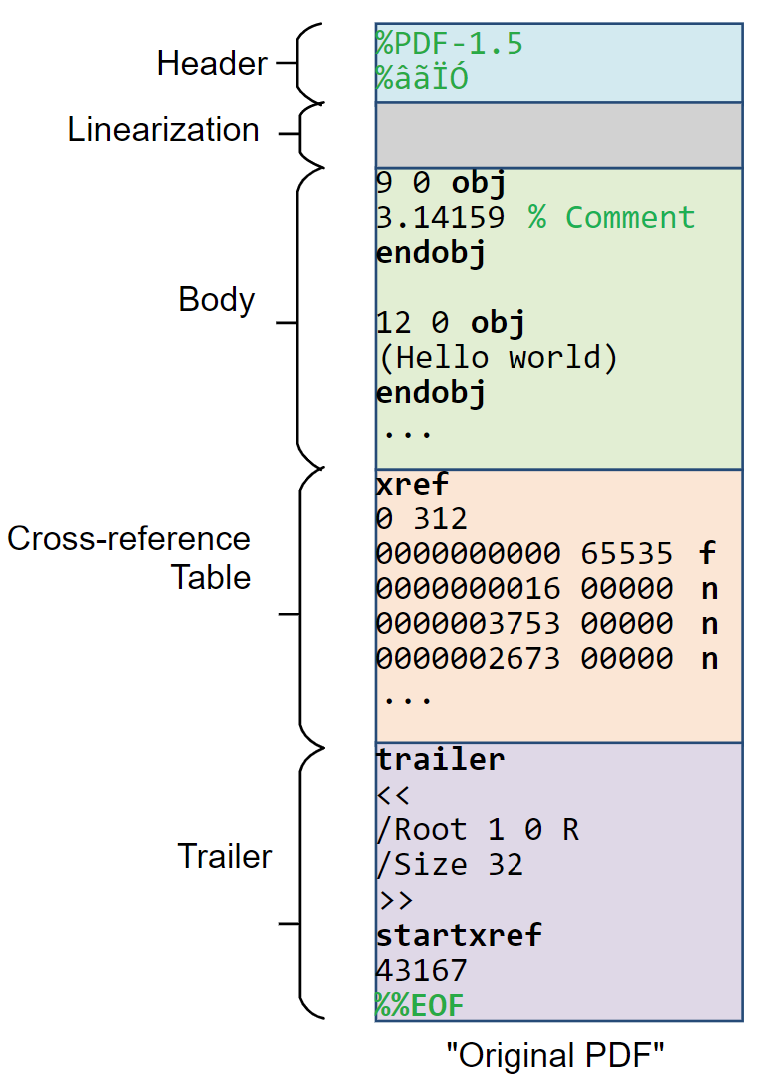
\includegraphics[width=0.35\linewidth]{figures/pdf-structure.png}
    \caption{PDF File Structure.}
    \label{fig:pdf-structure}
    \pwtodo{replace with better diagram}
\end{figure}

The overall structure of a PDF is shown in \cref{fig:pdf-structure}.

\pwtodo{short paragraph: describe overall PDF doc structure}

\pwtodo{more detail}

... and then locate either the \lstcd{xref} keyword for
traditional PDF cross-reference tables, or a PDF object that should be
a cross-reference stream.  In the case of traditional PDF
cross-reference tables, after the cross reference table will be the
trailer dictionary identified by the \lstcd{trailer} keyword or,
alternatively for PDF 1.5 and later files with cross-reference
streams, the trailer dictionary keys will be in the stream extent
dictionary of the cross reference stream.

... these are identified by a \lstcd{Prev} entry in either the trailer
dictionary or the stream extent dictionary of a cross-reference stream. The
value of the \lstcd{Prev} key is another byte offset to the immediately
preceding incremental update which, again, can either be a traditional
cross-reference table and to the start of the \lstcd{xref} keyword, or to a
cross-reference stream. This process repeats, working from the most recent
update back through time to the original PDF document.

Of particular note is the \lstcd{Size} entry, which
is one greater than the largest object number allocated in the PDF
file.

In this stage, data in each cross reference table must then be parsed to
identify the byte offset to the start of each PDF object. Note also that PDF
does not define the byte offset to the end of an object.

There are two sets of
objects in every PDF document: the in-use list of PDF objects and a free list
of PDF objects. Object zero is always the start of the free list as it is not
otherwise a valid object number.

For incremental updates, PDF object numbering
does not have to be sequential, with skipped object numbers assumed to be on
the free list (although this is not stated explicitly in the PDF
specification).

Parsing depends on the form of the incremental update, with
traditional cross-reference tables being simpler and largely independent of
other processing. Cross-reference streams however are more complex as they are
usually compressed and thus require the pre-DOM parser to "trust" the stream
extent dictionary data.

Each incremental update can add new objects, mark existing in-use objects as
free, or reinstate previously freed objects.


\mttodo{maybe: import the type definitions}

\subsection{Root Causes of PDF Complexity}

Most data formats can be described by much simpler mechanisms;
most language processors (e.g., a Python parser) can be described and parsed by
textbook methods (e.g., the old \emph{lex} and \emph{yacc} are sufficient for
most language processors);
so what makes PDF processing so much more complex?
\begin{lstlisting}[style=meta]
  - indirect offsets
    - which may recursively point to other indirect offsets
    - need programming language
      (or a 'seek' in the data definition lang)
  - DOM is a directed graph structure that allows cycles and arbitrary references (so not a DAG)
    - objects point to objects via byte offsets (cf. not by nested expressions such as XML)  
  - backwards parsing
  - incremental updates as a set of deltas to be applied to the file, which change the DOM
    - (note: unlike HTML, PDF's DOM is fixed and cannot be altered by JS)
  - XRef tables ...
  - ... giving rise to cavities
    - giving rise to polyglots
  - dependent parsers
\end{lstlisting}

\subsection{\todo{para. needs home: ``data integrity relationships...''}}

\todo{we should use the concept of "data integrity relationships" being the
  essence of the necessary context. e.g. PDF incremental updates are appended to
  a previously valid PDF - thus an incremental update should not "make visible"
  a PDF object that was not already valid and visible in the original PDF (this
  is one method Shadow Attacks use - cf. an upstream "supply chain attack" by an
  attacker), even if that PDF object is otherwise entirely syntactically
  valid. In the same way an incremental update that refers to an object at a
  file byte offset after the incremental update would be highly suspicious.}

% ------------------------------------------------------------------------------
\subsection{Vulnerabilities \note{1pp}}
\label{sec:vulnerabilities}

% As will become even more apparent, there is a significant amount of
% parsing and computation that needs to be done \emph{pre-DOM}.

Given our recent points about the \emph{PDF Trust Chain}
(\cref{sec:trust-chain}),
it should not surprise us that most of the PDF attack vectors
involve some aspect of breaking the \emph{DOM} abstraction.
I.e., the vulnerabilities occur \emph{pre-DOM}.

{\bf{Shadow Attacks}} \todo{...}

{\bf{Schizophrenia}} \todo{should define what we mean by schizo - is this the same thing that gives rise to parser differentials or a feature of of the syntax or layout of PDF?}
\begin{lstlisting}[style=meta]
  - writer errors
  - parser differentials
    - e.g., ignoring XRef tables
  - recovering parsers !!
  - blind faith in incremental updates (Shadow Attacks)
\end{lstlisting}

{\bf{Polyglots}} 
\todo{... arising from cavities and permissive implementations and ...}
\begin{lstlisting}[style=meta]
- Multiple places for hidden/unused/malicious data in PDF
  - non-obvious places, unnoticed when "simply parsing"
  - e.g., shadow-attacks
  - dead bytes, dead objects, dead updates, dead linearization sections, etc.
\end{lstlisting}

{\bf{Denial of Service (DOS)}} 
%
\begin{lstlisting}[style=meta]
- [potential recursion many places]
- format may not be well-defined because the recursion is not
    "well-defined"
\end{lstlisting}



{\bf{Others}} \todo{Maybe PII/redaction issues - just 'cos you delete something in a PDF doesn't mean it is really deleted (thanks to incremental updates)!!!! }

